\documentclass[10pt, a4paper]{article}
\usepackage[utf8]{inputenc}
\usepackage[frenchb]{babel}
\usepackage[OT1]{fontenc}
\usepackage{amsfonts, amsmath, amssymb, amsthm, dsfont, amsthm}
\usepackage{a4wide}
\usepackage[dvipsnames]{xcolor}
\usepackage{tikz} 
\usetikzlibrary{arrows,positioning,shapes}

\title{\textbf{Lab Report} \\ Week of 12/01/2016}
%\author{Olivier \textsc{Mangin}}
%\date{\today}

\definecolor{main}{named}{BurntOrange}
\definecolor{second}{named}{RoyalBlue}
%\newcommand{\maincolor}{orange}
%\newcommand{\secondcolor}{orange!20}
\newcommand{\strong}[1]{\textcolor{main}{\textbf{#1}}}
\newcommand{\stronger}[1]{\textcolor{second}{\textbf{#1}}}
\newcommand{\colored}[1]{\textcolor{main}{#1}}

% Affichage du titre avec les numéro et date de la semaine
\newcommand{\titre}[2]{
\noindent
\hspace{-10pt}
\begin{tabular}{lr}
  \hspace{0.58\textwidth} & \hspace{0.4\textwidth} \\
  \strong{\huge Lab Report} & \textbf{\Large #1} \medskip \\
  \textbf{\Large Name \& Roll} & {\large #2} ~\\
\end{tabular}

\vspace{20pt}
}

% Encadré ``En bref'' réumant les avancées et problèmes de la semaine
\newenvironment{enbref}{
\noindent\fcolorbox{main}{main}{
\begin{minipage}{\textwidth}
\textcolor{white}{\textbf{\large }}
\end{minipage}
} \\

}{
\begin{center}
  \strong{ \rule[2mm]{\textwidth}{3pt} }
\end{center}
\vspace*{-20pt}
}

% Affichage d'un titre de rubrique
\newcommand{\rubrique}[1]{
  \bigskip
  \begin{center}
  \begin{minipage}{\textwidth}
    \noindent\strong{{\large #1} \\
      \rule[2mm]{\textwidth}{1pt} }
  \end{minipage}
  \end{center}
  \vspace*{-20pt}
}

% Symbole utilisé en début de ligne des éléments
\newcommand{\doublerect}{
\begin{tikzpicture}
  \fill[color=main] (0,0) rectangle (4pt,-4pt);
  \fill[color=second] (2pt,-2pt) rectangle (6pt,-6pt);
\end{tikzpicture}
}

% Affichage d'un titre d'élément
\newcommand{\element}[1]{
  \medskip
  \noindent\textcolor{second}{ \doublerect \textbf{#1}}
}

% Pour les lectures, petit raccourci pour mettre en avant le niveau
% de lecture d'un article.
\newcommand{\lu}{\strong{[Lu]} }
\newcommand{\parcouru}{\strong{[Parcouru]} }
\newcommand{\alire}{\strong{[A lire]} }
\newcommand{\presentation}{\strong{[Présentation]} }
\newcommand{\keynote}{\strong{[Keynote]} }



\usepackage[pdfauthor={Name}, pdftitle={Weekly}, pdfsubject={Week 1}, pdfkeywords={},colorlinks=true,urlcolor=black,linkcolor=black, citecolor=black]{hyperref}
\usepackage{listings}
\usepackage{subfig}
\usepackage{graphicx}
\lstset{%
language=Matlab,
frame=single,
%numbers=left,
%numberstyle=\footnotesize,
%tabsize=2,
keepspaces=true,
columns=fullflexible,
basicstyle=\ttfamily\scriptsize,
keywordstyle=\color{blue}
}


\begin{document}

\renewcommand{\labelitemi}{\textcolor{main}{\small $\blacktriangleright$}}
\renewcommand{\labelitemii}{\textcolor{second}{\scriptsize \textbullet}}

\titre{Week 7}{06/03/2017}

\begin{enbref}
\element{Title}
\begin{itemize}
\item Implement the Sutherland-Hodgeman algorithm for polygon clipping.\\
    1). OpenGL\\
    2). MatLab
\end{itemize}
\medskip
\end{enbref}

\rubrique{Procedure}
\vspace{0.5mm} \flushleft

\element {OpenGL}

\vspace{0.5mm} \flushleft
1). Choose N vertices of a polygon and define a clipping window and then apply the algorithm    described below :
\begin{itemize}
\item Create a C file and name it as \textit{polygonclipping.c}.
\item Following is the final code for Sutherland-Hodgeman algorithm for polygon clipping :
\begin{lstlisting}
#include <math.h>
#include <stdio.h>
#include <string.h>
#include <stdlib.h>
#include <assert.h>
#include <limits.h>
#include <stdbool.h>
#include <ctype.h>
#include <GL/glut.h>

double x_min=10 , x_max=50, y_min=10, y_max=50;
int i = 0; int number_of_vertices = 5;
double xcoordinates[7];
double ycoordinates[7];

double xf1 = 0; double yf1 = 0 ;
double xf2 = 0 ; double yf2 = 0 ;

int get_code_for_this_point(float x,float y)
{
        int c=0;
        if(y>y_max) c=8;
        if(y<y_min) c=4;
        if(x>x_max) c=c|2;
        if(x<x_min) c=c|1;
        return c;
}

void clipping_Line(float x1,float y1,float x2,float y2)
{
        int c1=get_code_for_this_point(x1,y1);
        int c2=get_code_for_this_point(x2,y2);

        while((c1|c2) != 0)
        {
                if((c1&c2) > 0)
                {
                        break;
                }

                float slope = (y2-y1)/(x2-x1);

                float xi = x1 ;
                float yi = y1 ;
                int code = c1 ;

                if(code==0)
                {
                    code = c2 ;
                    xi = x2 ;
                    yi = y2 ;
                }

                float x = 0 ; float y = 0;

                if((code & 8)>0)
                {
                        y = y_max;
                        x = xi+ 1.0/slope*(y_max-yi);
                }
                else if((code & 4)>0)
                {
                    y = y_min;
                    x = xi+1.0/slope*(y_min-yi);
                }
                else if((code & 2)>0)
                {
                    x = x_max;
                    y = yi+slope*(x_max-xi);
                }
                else if((code & 1)>0)
                {
                    x = x_min;
                    y = yi+slope*(x_min-xi);
                }

                if(code == c1)
                {
                    xf1 = x ;
                    yf1 = y ;
                    c1 = get_code_for_this_point(xf1,yf1);
                }
                if(code == c2)
                {
                    xf2 = x ;
                    yf2 = y ;
                    c2 = get_code_for_this_point(xf2,yf2);
                }
        }
}

void display_function_after()
{
        glClearColor(1.0, 1.0, 1.0, 1.0);
        glClear(GL_COLOR_BUFFER_BIT);
        glLineWidth(3);
        glBegin(GL_LINES);
                glColor3f(0.0f, 0.0f, 0.0f);
                glVertex2f(0.0f,400.0f);
                glVertex2f(0.0f,-400.0f);
                glVertex2f(400.0f,0.0f);
                glVertex2f(-400.0f,0.0f);
        glEnd();

        glLineWidth(3);
        glBegin(GL_LINE_LOOP);
                glColor3f(1.0f, 0.0f, 0.0f);
                glVertex2f(x_min/100.0f,y_min/100.0f);
                glVertex2f(x_max/100.0f,y_min/100.0f);
                glVertex2f(x_max/100.0f,y_max/100.0f);
                glVertex2f(x_min/100.0f,y_max/100.0f);
        glEnd();
        glLineWidth(3);
        for(i = 0 ; i < number_of_vertices ; i++)
        {
                xf1 = xcoordinates[i];
                yf1 = ycoordinates[i];
                xf2 = xcoordinates[i+1];
                yf2 = ycoordinates[i+1];
                clipping_Line(xf1,yf1,xf2,yf2);
                glBegin(GL_LINES);
                    glColor3f(0.0f, 0.0f,1.0f);
                    glVertex2f(xf1/100.0f,yf1/100.0f);
                    glVertex2f(xf2/100.0f,yf2/100.0f);
                glEnd();
        }
}
void display_function_before()
{
        glClearColor(1.0, 1.0, 1.0, 1.0);
        glClear(GL_COLOR_BUFFER_BIT);
                glLineWidth(3);
                glBegin(GL_LINES);
                    glColor3f(0.0f, 0.0f, 0.0f);
                    glVertex2f(0.0f,400.0f);
                    glVertex2f(0.0f,-400.0f);
                    glVertex2f(400.0f,0.0f);
                    glVertex2f(-400.0f,0.0f);
                glEnd();

                glLineWidth(3);
                glBegin(GL_LINE_LOOP);
                    glColor3f(1.0f, 0.0f, 0.0f);
                    glVertex2f(x_min/100.0f,y_min/100.0f);
                    glVertex2f(x_max/100.0f,y_min/100.0f);
                    glVertex2f(x_max/100.0f,y_max/100.0f);
                    glVertex2f(x_min/100.0f,y_max/100.0f);
                glEnd();

                glLineWidth(3);
                glBegin(GL_LINE_LOOP);
                    glColor3f(0.0f, 0.0f, 1.0f);
                        for(i = 0 ; i < number_of_vertices ; i++)
                        {
                                glVertex2f(xcoordinates[i]/100.0f,ycoordinates[i]/100.0f);
                        }
                glEnd();

            glFlush();
        glutSwapBuffers();
}
int main(int argc, char const *argv[])
{
        glutInit(&argc,argv);
        glutInitDisplayMode(GLUT_RGB);
        glutInitWindowSize(500, 500);
        gluOrtho2D(-400, 400, -400, 400);
        xcoordinates[0] = 5 ; xcoordinates[1] = 30; xcoordinates[2] = 40 ; xcoordinates[3] = 55; xcoordinates[4] = 30;
        xcoordinates[5] = 5;
        ycoordinates[0] = 30; ycoordinates[1] = 5; ycoordinates[2] = 30; ycoordinates[3] = 30; ycoordinates[4] = 55;
        ycoordinates[5] = 30 ;
        glutCreateWindow("Sutherland-Hodgman Polygon Clipping: Before");
        glutDisplayFunc(display_function_before);
        glutCreateWindow("Sutherland-Hodgman Polygon Clipping: After");
        glutDisplayFunc(display_function_after);
        glutMainLoop();
        return 0;
}
\end{lstlisting}

\vspace{0.5mm}

\item Compile and run the executable file in terminal by typing in the following commands : \\

\vspace{0.5mm} \flushleft

\textit{(a)\hspace{2mm} gcc polygonClipping.c -lGL -lGLU -lglut -ll} \\
\textit{(b)\hspace{2mm} ./a.out}
\vspace*{1\baselineskip}
\end{itemize}

\element {MatLab}\\

1). Choose N Vertices of a polygon and define a clipping window and then apply the algorithm described below :

\begin{itemize}

\item Open a new matlab script and define a function polygonClipping().
\item Following is the final code for Sutherland-Hodgman algorithm for polygon clipping.
\begin{lstlisting}

function m = polygonClipping()
        X = [5,30,40,55,30,5];
        Y = [30,5,30,30,55,30];
        pointsX = [];
        pointsY = [];
        xmin=10; xmax=50; ymin=10 ; ymax=50 ;
        boundries_x = [xmin,xmax,xmax,xmin,xmin];
        boundries_y = [ymin,ymin,ymax,ymax,ymin];
        plot(boundries_x, boundries_y, 'g-', 'LineWidth', 3);
        hold on;
        for i = 1:5
                [pointsX,pointsY] = Clipping(X(i),Y(i),X(i+1),Y(i+1),xmin, ymin, xmax, ymax,pointsX,pointsY);
        end
        pointsX = [pointsX pointsX(1)];
        pointsY = [pointsY pointsY(1)];
        plot(pointsX, pointsY, 'b-', 'LineWidth', 3);
end
function [pointsX,pointsY] = Clipping(xf1 , yf1 , xf2 , yf2 , xmin, ymin, xmax, ymax,pointsX,pointsY)
        plot([xf1 xf2], [yf1 yf2], 'r--','LineWidth', 3);
        hold on;
        code1 = code(xf1, yf1, xmin, xmax, ymin, ymax);
        code2 = code(xf2, yf2, xmin, xmax, ymin, ymax);

                if bitand(code1,code2) > 0

                end

        while bitor(code1,code2) > 0

                slope  = (yf2-yf1)/(xf2-xf1);
                codex = code1 ;
                xi = xf1 ;
                yi = yf1 ;

                if(codex==0)
                        codex = code2;
                        xi = xf2 ;
                        yi = yf2 ;
                end

                if bitand(codex,8)>0
                        y = ymax;
                        x = xi + 1/slope*(ymax-yi);
                elseif bitand(codex,4)>0
                        y = ymin ;
                        x = xi + 1/slope*(ymin-yi);
                elseif bitand(codex,2)>0
                        x = xmax;
                        y = yi + slope*(xmax-xi);
                elseif bitand(codex,1)>0
                        x = xmin;
                        y = yi + slope*(xmin-xi);
                end

                if codex == code1
                        xf1 = x;
                        yf1 = y;
                        code1 = code(xf1, yf1, xmin, xmax, ymin, ymax);
                elseif codex == code2
                        xf2 = x ;
                        yf2 = y ;
                        code2 = code(xf2, yf2, xmin, xmax, ymin, ymax);
                end
        end
        pointsX = [pointsX xf1];
        pointsX = [pointsX xf2];
        pointsY = [pointsY yf1];
        pointsY = [pointsY yf2];
end
function c = code(xf2, yf2, xmin, xmax, ymin, ymax)
        c = 0;
        if (yf2>ymax)
                c = 8;
        end
        if (yf2<ymin)
                c = 4;
        end
        if (xf2>xmax)
                c = bitor(c,2);
        end
        if (xf2<xmin)
                c = bitor(c,1);
        end
end

\end{lstlisting}
\end{itemize}
\rubrique{Output}
\begin{figure}[ht!]
\centering
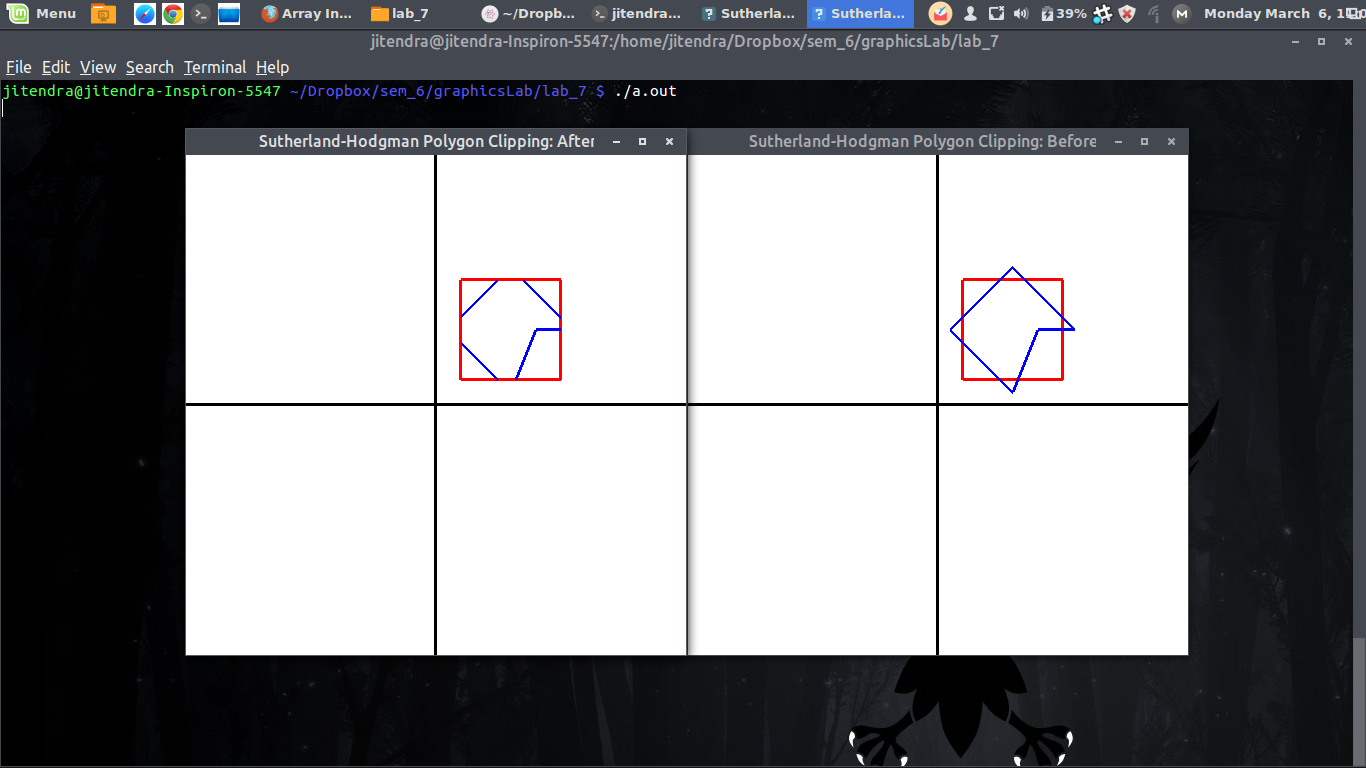
\includegraphics[width=150mm, height=100mm]{polygonClippingOpenGL.png}
\caption{Sutherland-Hodgman polygon clipping in OpenGL \label{overflow}}
\end{figure}
\begin{figure}[ht!]
\centering
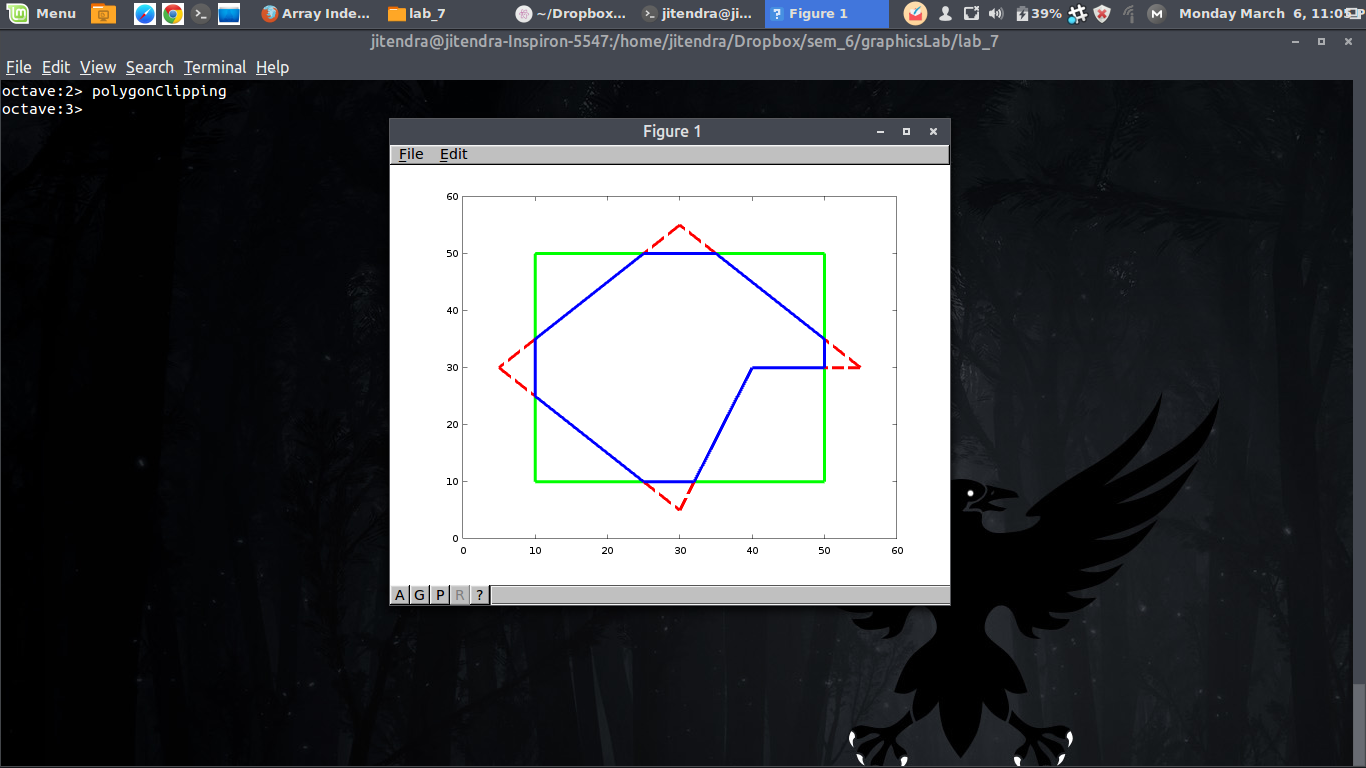
\includegraphics[width=150mm, height=100mm]{polygonClippingMatlab.png}
\caption{Sutherland-Hodgman Polygon clipping in Matlab \label{overflow}}
\end{figure}
\end{document}
